\chapter{Introduction}
% See Joel page 3 for 3 main difficulties of EDL
%
%
\section{Motivation}

\section{Dissertation Goals}
%\section{Literature Review?}

% Mars entry problem - mission requirements and future stuff

% State of practice - MSL/M2020

% Covariance reduction based entry guidance - also discussion of sensivity based approaches and comparison work. Also terminology: robust OCP versus optim under unc versus...

% Introduction to my approach? 
% State the specific objective(s) of my research 


We demonstrate that, with a reformulation of the objective function, the robust optimal control problem can be solved using differential dynamic programming (DDP) \cite{DDP}, a shooting method originally devised to solve unconstrained nonlinear optimal control problems that has since seen numerous extensions, including to constrained problems \cite{DDP_ControlLimited,HDDP1,HDDP2,DDP_NonlinearConstraints,DDP_InteriorPoint}, and stochastic problems \cite{iLQG, DDP_Stochastic, ozaki_UT,ozaki2020tube}. 
Starting from the control-limited DDP algorithm \cite{DDP_ControlLimited}, we examine a iterated Linear-Quadratic-like simplification \cite{iLQG} that enables solution of large-scale optimal control problems. Next, we extend the algorithm to jointly optimize the static feedback gains along with the reference control.

% TODO: Talk about related work 
%Due to the interest in high elevation landings, guidance algorithms designed to maximize altitude at parachute deploy have been studied using optimal control theory 
%\cite{AltitudeOptimization,AltitudeOptimizationIndirect}. Reference \cite{GuangfeiDissertation} proposed an optimization-based onboard trajectory planning method based on a low-order parametrization designed to achieve high altitude at parachute deploy.
%Typically these papers consider predictive guidance and use parametrizations of the bank angle designed to yield high altitudes. 

% Refences with notes:
% AltitudeUnderUncertainty
% MarsEntryDesensitized % linearized but closed-loop with fixed gain. No consideration of saturation 
% EntryOUU % Does not use linearization, also doesnt solve in a conventional way, maybe remove?
% TrajectoryDesensitization % Desensitized like seywald and kumar, is it entry applied?
% EntryOUUThesis1 % Earth EDL, focuses on footprint computation, only considers open-loop in the reentry problem, and did not conduct monte carlo to confirm
% EntryOUUThesis2 % LQR, minimum control effort objective which stays away from the bounds, angle of attack as control variable. Does perform Monte Carlo(s) to validate improvement. 

Throughout this dissertation, we refer to optimal control formulations that weight a nominal (or mean) optimization objective with minimization of covariance terms as robust optimal control. The nomenclature in the literature also sometimes refer to such problems as uncertain optimal control \cite{PhelpsUncertainOCP}, optimal control under uncertainty. Due to the close relationship between the sensitivity matrix (also called the state transition matrix) and the covariance matrix, we also include desensitized optimal control \cite{Desensitized,TrajectoryDesensitization} under the umbrella of robust optimal control. 
Approaches to entry guidance based on robust optimal control have been studied in \cite{AltitudeUnderUncertainty, EntryOUUThesis1, EntryOUUThesis2, MarsEntryDesensitized, EntryOUU}. Reference~\cite{EntryOUUThesis1} explored the relationship between covariance reduction and sensitivity reduction, and ultimately recommended the covariance formulation for several reasons, including smaller problem size due to the symmetry of the covariance matrix, the ability to incorporate measurements, and simpler formulation and interpretation of variances compared to elements of the sensitivity matrix.

The works most closely related to our approach are Ref.~\cite{AltitudeUnderUncertainty}, where the objective was to maximize a function of the mean and standard deviation of altitude, and Ref.~\cite{MarsEntryDesensitized}, where the objective was to maximize terminal altitude while penalizing sensitivity terms related to variations in the initial state. Compared to Ref.~\cite{AltitudeUnderUncertainty}, our work differs by considering a multi-objective formulation that includes a downrange performance objective rather than strictly focusing on altitude, by considering closed-loop dynamics instead of open-loop, and by using the unscented transform instead of linear covariance propagation. Similarly, Ref.~\cite{MarsEntryDesensitized} also employed linear covariance propagation, but did consider closed-loop performance with fixed feedback gains. Their method made use of sensitivities, rather than statistics, in order to increase robustness to off-nominal situations. Additionally, a single penalty factor was applied to all terminal state sensitivities, including flight path angle. In contrast, we penalize only altitude and downrange deviations, and use a separate penalty factor for each component. An additional difference is that we consider parametric uncertainty in the equations of motion rather than solely uncertainty in the initial state. 

\begin{figure}[h!]
	\centering
	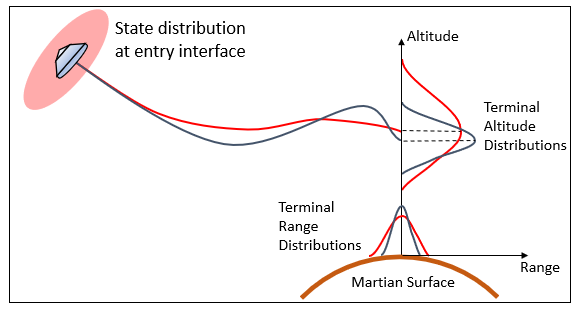
\includegraphics[width=1\textwidth]{Images/RobustTrajectoryOptimization}
	\caption{Comparison of UQ methods in an closed-loop scenario}
	\label{Fig:RobustTrajectoryOpt}
\end{figure}
%The specific objective of this dissertation are to design an entry guidance with the same computational complexity as the state-of-the-practice guidance algorithm while providing superior performance. 

\section{Dissertation Organization}
This remainder of this dissertation is organized as follows: \\
Chapter two discusses the dynamics and models used to derive the guidance algorithm\\
Chapter three describes the entry guidance problem, especially target condition(s)\\
Chapter four outlines the guidance strategy, including posing the problem as a ROCP. Gain optimization (or selection) as well. \\
Chapter five gives an algorithm based on constrained DDP/SLQ to solve the ROCP; Also UQ and reformulations; demonstration of open-loop vs closed loop necessity of UT \\
Chapter six presents the assessment conditions (simulation details, Monte Carlo) Maybe UT-alpha choice should be discussed here?\\
Chapter seven presents an assessment of the guidance algorithm. Choice of alpha parameter. Problems with joint optimization as well (UT cov almost zero but MC cov bad) \\
Chapter eight concludes the dissertation \\

%chapter details two extensions to the DDP algorithm - an augmented lagrangian method for enforcing terminal constraints and a method for optimizing (constant) parameters, such as the feedback gains (lateral corridor params? probably not due to differentiable req) and the initial flight path angle. The gain optimization in particular is important because of the issue with joint optimization of time-varying gains. 

%%% Local Variables: ***
%%% mode: latex ***
%%% TeX-master: "thesis.tex" ***
%%% End: ***
